\documentclass[handout,nooutcomes]{ximera}
%% handout
%% space
%% newpage
%% numbers
%% nooutcomes


\newcommand{\RR}{\mathbb R}
\renewcommand{\d}{\,d}
\newcommand{\dd}[2][]{\frac{d #1}{d #2}}
\renewcommand{\l}{\ell}
\newcommand{\ddx}{\frac{d}{dx}}
\newcommand{\dfn}{\textbf}
\newcommand{\eval}[1]{\bigg[ #1 \bigg]}

\usepackage{multicol}

\renewenvironment{freeResponse}{
\ifhandout\setbox0\vbox\bgroup\else
\begin{trivlist}\item[\hskip \labelsep\bfseries Solution:\hspace{2ex}]
\fi}
{\ifhandout\egroup\else
\end{trivlist}
\fi} %% we can turn off input when making a master document

\title{Recitation \#2 Chapter 1 - Precalculus Review}  

\begin{document}
\begin{abstract}		\end{abstract}
\maketitle

\section*{Warm up:}
   
If $f$ is always increasing, is $f^{-1}$ always increasing?


\section*{Group work:}
	\begin{problem}
	 	Given the graph of the function $f$ below, answer the following questions.
			
\begin{image}		
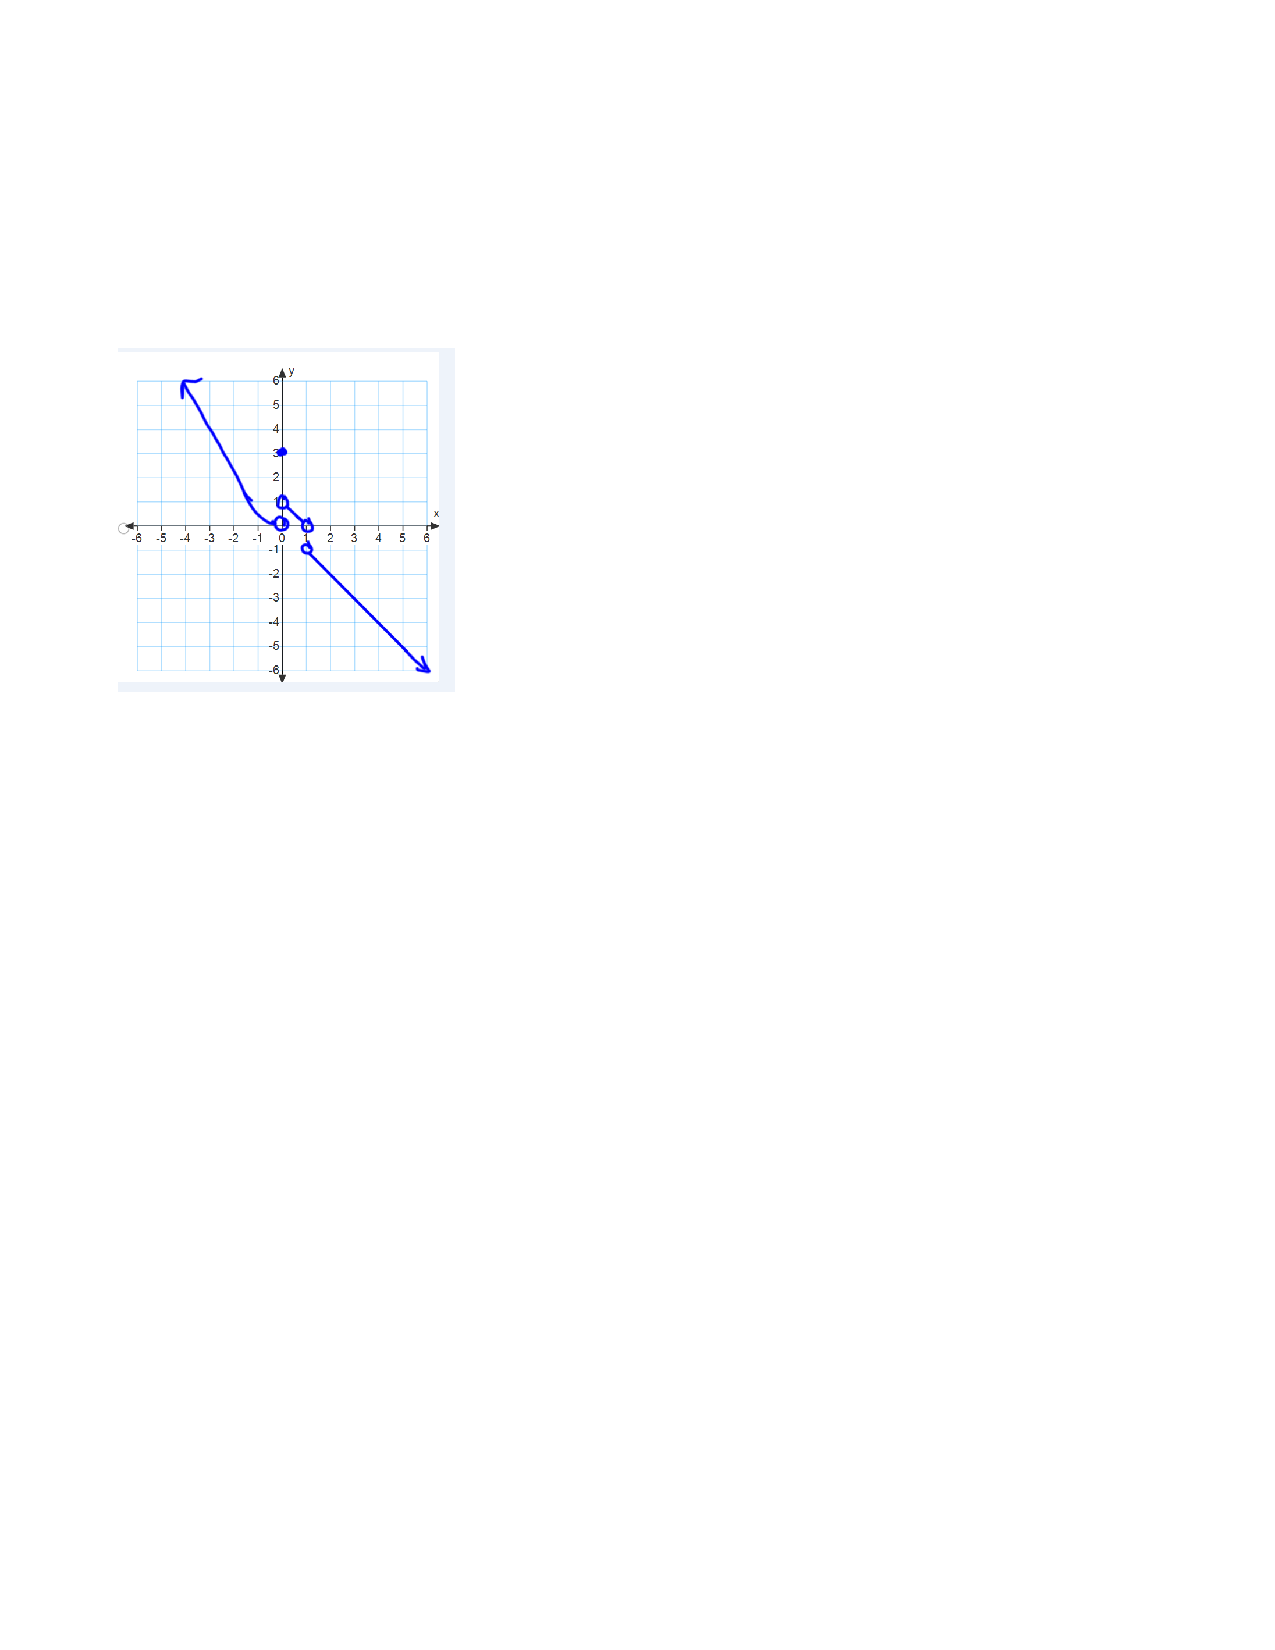
\includegraphics[trim= 80 460 300 170]{Figure3.pdf}
\end{image}	

		\begin{enumerate}
		
			 \item What is the domain of $f$?
			 
			 \begin{freeResponse}
			 
			 $(-\infty, 1)$ and $(1, \infty)$
	
			\end{freeResponse}
			 
			 \item What is the range of $f$?
			 
			 \item What is $f(0)$?  $f(1)$?  $f(2)$?
			 
			 \item Does $f$ have an inverse?  Why or why not?
			
			\end{enumerate}
			
	\begin{freeResponse}
	
	\end{freeResponse}
			
	\end{problem}
	
	\begin{enumerate}
			
				
	\item  Find the inverse $y=f^{-1}(x)$ of the function.  State the domain and range of the inverse.
	
			\begin{enumerate}
			\item  $f(x)=x^2-4x-5$ (when $x>2$).
			\item  $f(x)=\sqrt[4]{x+2}$.
			\item  $f(x)=\frac{1}{(x+2)^2}$  (when $x>2$).
			\end{enumerate}
	
	
	
	\item  Find all values of $x$ which satisfy the equation.
	
			\begin{enumerate}
			
			\item  $\log_x 25=2$ 
			
			\item  $7^x=15$ 
			
			\end{enumerate}
			
			
			\item  Find all values which satisfy the given equation.
	
			\begin{enumerate}
			
			\item  $\cos (x)=1$ 
			
			\item  $\sin (3 \theta )=\frac{\sqrt{3}}{2}$ for $0 \leq \theta \leq 2\pi $
			
			\end{enumerate}
			
			
			
	\item
	
			\begin{enumerate}
			
			\item  Simplify the expression:  $\cos^{-1} \left( \sin \left( \frac{\pi }{2} \right) \right) $ 
			
			\item  Simplify the expression:  $ \tan \left( \cos^{-1} \left( \frac{4}{x} \right) \right) $ 
			
			\end{enumerate}
			
			
			

	










								
				
				
	\end{enumerate}



























\end{document} 


















